\documentclass[]{article}
\usepackage{lmodern}
\usepackage{amssymb,amsmath}
\usepackage{ifxetex,ifluatex}
\usepackage{fixltx2e} % provides \textsubscript
\ifnum 0\ifxetex 1\fi\ifluatex 1\fi=0 % if pdftex
  \usepackage[T1]{fontenc}
  \usepackage[utf8]{inputenc}
\else % if luatex or xelatex
  \ifxetex
    \usepackage{mathspec}
    \usepackage{xltxtra,xunicode}
  \else
    \usepackage{fontspec}
  \fi
  \defaultfontfeatures{Mapping=tex-text,Scale=MatchLowercase}
  \newcommand{\euro}{€}
\fi
% use upquote if available, for straight quotes in verbatim environments
\IfFileExists{upquote.sty}{\usepackage{upquote}}{}
% use microtype if available
\IfFileExists{microtype.sty}{%
\usepackage{microtype}
\UseMicrotypeSet[protrusion]{basicmath} % disable protrusion for tt fonts
}{}
\usepackage[margin=1in]{geometry}
\ifxetex
  \usepackage[setpagesize=false, % page size defined by xetex
              unicode=false, % unicode breaks when used with xetex
              xetex]{hyperref}
\else
  \usepackage[unicode=true]{hyperref}
\fi
\hypersetup{breaklinks=true,
            bookmarks=true,
            pdfauthor={John Slough II},
            pdftitle={Practical Machine Learning Project: Weight Lifting Exercise Classification},
            colorlinks=true,
            citecolor=blue,
            urlcolor=blue,
            linkcolor=magenta,
            pdfborder={0 0 0}}
\urlstyle{same}  % don't use monospace font for urls
\usepackage{color}
\usepackage{fancyvrb}
\newcommand{\VerbBar}{|}
\newcommand{\VERB}{\Verb[commandchars=\\\{\}]}
\DefineVerbatimEnvironment{Highlighting}{Verbatim}{commandchars=\\\{\}}
% Add ',fontsize=\small' for more characters per line
\usepackage{framed}
\definecolor{shadecolor}{RGB}{248,248,248}
\newenvironment{Shaded}{\begin{snugshade}}{\end{snugshade}}
\newcommand{\KeywordTok}[1]{\textcolor[rgb]{0.13,0.29,0.53}{\textbf{{#1}}}}
\newcommand{\DataTypeTok}[1]{\textcolor[rgb]{0.13,0.29,0.53}{{#1}}}
\newcommand{\DecValTok}[1]{\textcolor[rgb]{0.00,0.00,0.81}{{#1}}}
\newcommand{\BaseNTok}[1]{\textcolor[rgb]{0.00,0.00,0.81}{{#1}}}
\newcommand{\FloatTok}[1]{\textcolor[rgb]{0.00,0.00,0.81}{{#1}}}
\newcommand{\ConstantTok}[1]{\textcolor[rgb]{0.00,0.00,0.00}{{#1}}}
\newcommand{\CharTok}[1]{\textcolor[rgb]{0.31,0.60,0.02}{{#1}}}
\newcommand{\SpecialCharTok}[1]{\textcolor[rgb]{0.00,0.00,0.00}{{#1}}}
\newcommand{\StringTok}[1]{\textcolor[rgb]{0.31,0.60,0.02}{{#1}}}
\newcommand{\VerbatimStringTok}[1]{\textcolor[rgb]{0.31,0.60,0.02}{{#1}}}
\newcommand{\SpecialStringTok}[1]{\textcolor[rgb]{0.31,0.60,0.02}{{#1}}}
\newcommand{\ImportTok}[1]{{#1}}
\newcommand{\CommentTok}[1]{\textcolor[rgb]{0.56,0.35,0.01}{\textit{{#1}}}}
\newcommand{\DocumentationTok}[1]{\textcolor[rgb]{0.56,0.35,0.01}{\textbf{\textit{{#1}}}}}
\newcommand{\AnnotationTok}[1]{\textcolor[rgb]{0.56,0.35,0.01}{\textbf{\textit{{#1}}}}}
\newcommand{\CommentVarTok}[1]{\textcolor[rgb]{0.56,0.35,0.01}{\textbf{\textit{{#1}}}}}
\newcommand{\OtherTok}[1]{\textcolor[rgb]{0.56,0.35,0.01}{{#1}}}
\newcommand{\FunctionTok}[1]{\textcolor[rgb]{0.00,0.00,0.00}{{#1}}}
\newcommand{\VariableTok}[1]{\textcolor[rgb]{0.00,0.00,0.00}{{#1}}}
\newcommand{\ControlFlowTok}[1]{\textcolor[rgb]{0.13,0.29,0.53}{\textbf{{#1}}}}
\newcommand{\OperatorTok}[1]{\textcolor[rgb]{0.81,0.36,0.00}{\textbf{{#1}}}}
\newcommand{\BuiltInTok}[1]{{#1}}
\newcommand{\ExtensionTok}[1]{{#1}}
\newcommand{\PreprocessorTok}[1]{\textcolor[rgb]{0.56,0.35,0.01}{\textit{{#1}}}}
\newcommand{\AttributeTok}[1]{\textcolor[rgb]{0.77,0.63,0.00}{{#1}}}
\newcommand{\RegionMarkerTok}[1]{{#1}}
\newcommand{\InformationTok}[1]{\textcolor[rgb]{0.56,0.35,0.01}{\textbf{\textit{{#1}}}}}
\newcommand{\WarningTok}[1]{\textcolor[rgb]{0.56,0.35,0.01}{\textbf{\textit{{#1}}}}}
\newcommand{\AlertTok}[1]{\textcolor[rgb]{0.94,0.16,0.16}{{#1}}}
\newcommand{\ErrorTok}[1]{\textcolor[rgb]{0.64,0.00,0.00}{\textbf{{#1}}}}
\newcommand{\NormalTok}[1]{{#1}}
\usepackage{graphicx,grffile}
\makeatletter
\def\maxwidth{\ifdim\Gin@nat@width>\linewidth\linewidth\else\Gin@nat@width\fi}
\def\maxheight{\ifdim\Gin@nat@height>\textheight\textheight\else\Gin@nat@height\fi}
\makeatother
% Scale images if necessary, so that they will not overflow the page
% margins by default, and it is still possible to overwrite the defaults
% using explicit options in \includegraphics[width, height, ...]{}
\setkeys{Gin}{width=\maxwidth,height=\maxheight,keepaspectratio}
\setlength{\parindent}{0pt}
\setlength{\parskip}{6pt plus 2pt minus 1pt}
\setlength{\emergencystretch}{3em}  % prevent overfull lines
\providecommand{\tightlist}{%
  \setlength{\itemsep}{0pt}\setlength{\parskip}{0pt}}
\setcounter{secnumdepth}{0}

%%% Use protect on footnotes to avoid problems with footnotes in titles
\let\rmarkdownfootnote\footnote%
\def\footnote{\protect\rmarkdownfootnote}

%%% Change title format to be more compact
\usepackage{titling}

% Create subtitle command for use in maketitle
\newcommand{\subtitle}[1]{
  \posttitle{
    \begin{center}\large#1\end{center}
    }
}

\setlength{\droptitle}{-2em}
  \title{Practical Machine Learning Project: Weight Lifting Exercise
Classification}
  \pretitle{\vspace{\droptitle}\centering\huge}
  \posttitle{\par}
  \author{John Slough II}
  \preauthor{\centering\large\emph}
  \postauthor{\par}
  \predate{\centering\large\emph}
  \postdate{\par}
  \date{12 July 2015}

\usepackage{graphicx}

% Redefines (sub)paragraphs to behave more like sections
\ifx\paragraph\undefined\else
\let\oldparagraph\paragraph
\renewcommand{\paragraph}[1]{\oldparagraph{#1}\mbox{}}
\fi
\ifx\subparagraph\undefined\else
\let\oldsubparagraph\subparagraph
\renewcommand{\subparagraph}[1]{\oldsubparagraph{#1}\mbox{}}
\fi

\begin{document}
\maketitle

\textbf{Introduction}

This project is concerned with identifying the execution type of an
exercise, the Unilateral Dumbbell Biceps Curl. The dataset includes
readings from motion sensors on participants bodies'. These readings
will be used to classify the performed exercise into five categories:
exactly according to the specification (Class A), throwing the elbows to
the front (Class B), lifting the dumbbell only halfway (Class C),
lowering the dumbbell only halfway (Class D) and throwing the hips to
the front (Class E). Please see the website
\url{http://groupware.les.inf.puc-rio.br/har} for more information.

\textbf{The Data}

Processing:

\begin{Shaded}
\begin{Highlighting}[]
\CommentTok{#setwd("~/Desktop/Courses/Coursera/Machine Learning/Project")}

\KeywordTok{library}\NormalTok{(caret)}
\end{Highlighting}
\end{Shaded}

\begin{verbatim}
## Loading required package: lattice
## Loading required package: ggplot2
\end{verbatim}

\begin{Shaded}
\begin{Highlighting}[]
\KeywordTok{library}\NormalTok{(randomForest)}
\end{Highlighting}
\end{Shaded}

\begin{verbatim}
## randomForest 4.6-10
## Type rfNews() to see new features/changes/bug fixes.
\end{verbatim}

\begin{Shaded}
\begin{Highlighting}[]
\KeywordTok{library}\NormalTok{(ggthemes)}
\KeywordTok{library}\NormalTok{(gridExtra)}
\KeywordTok{library}\NormalTok{(ggplot2)}
\KeywordTok{library}\NormalTok{(grid)}
\NormalTok{train =}\StringTok{ }\KeywordTok{read.csv}\NormalTok{(}\StringTok{"pml-training.csv"}\NormalTok{,}\DataTypeTok{header=}\OtherTok{TRUE}\NormalTok{)}
\NormalTok{train_used =}\StringTok{ }\NormalTok{train[,}\KeywordTok{c}\NormalTok{(}\DecValTok{8}\NormalTok{:}\DecValTok{11}\NormalTok{,}\DecValTok{37}\NormalTok{:}\DecValTok{49}\NormalTok{,}\DecValTok{60}\NormalTok{:}\DecValTok{68}\NormalTok{,}\DecValTok{84}\NormalTok{:}\DecValTok{86}\NormalTok{,}\DecValTok{102}\NormalTok{,}\DecValTok{113}\NormalTok{:}\DecValTok{124}\NormalTok{,}\DecValTok{140}\NormalTok{,}\DecValTok{151}\NormalTok{:}\DecValTok{160}\NormalTok{)]}
\end{Highlighting}
\end{Shaded}

The raw dataset contained \(19622\) rows of data, with \(160\)
variables. Many variables contained largely missing data (usually with
only one row of data), so these were removed from the dataset (these
variables were also not used in the final 20 testing dataset). In
addition, variables not concerning the movement sensors were also
removed. This resulted in a dataset of \(53\) variables.

To understand the structure of the data a bit better, density plots were
made of a selection of the data. These are displayed below.

\begin{Shaded}
\begin{Highlighting}[]
\NormalTok{A=}\KeywordTok{ggplot}\NormalTok{() +}\StringTok{ }\KeywordTok{geom_density}\NormalTok{(}\KeywordTok{aes}\NormalTok{(}\DataTypeTok{x=}\NormalTok{gyros_belt_x), }\DataTypeTok{colour=}\StringTok{"red"}\NormalTok{, }\DataTypeTok{data=}\NormalTok{train_used) +}\StringTok{ }
\StringTok{  }\KeywordTok{geom_density}\NormalTok{(}\KeywordTok{aes}\NormalTok{(}\DataTypeTok{x=}\NormalTok{gyros_belt_y), }\DataTypeTok{colour=}\StringTok{"green"}\NormalTok{, }\DataTypeTok{data=}\NormalTok{train_used)+}
\StringTok{  }\KeywordTok{geom_density}\NormalTok{(}\KeywordTok{aes}\NormalTok{(}\DataTypeTok{x=}\NormalTok{gyros_belt_z), }\DataTypeTok{colour=}\StringTok{"blue"}\NormalTok{, }\DataTypeTok{data=}\NormalTok{train_used)+}
\StringTok{  }\KeywordTok{theme_few}\NormalTok{()+}\KeywordTok{xlab}\NormalTok{(}\StringTok{"Gyro Belt (xyz)"}\NormalTok{)}

\NormalTok{B=}\KeywordTok{ggplot}\NormalTok{() +}\KeywordTok{geom_density}\NormalTok{(}\KeywordTok{aes}\NormalTok{(}\DataTypeTok{x=}\NormalTok{roll_belt), }\DataTypeTok{colour=}\StringTok{"red"}\NormalTok{, }\DataTypeTok{data=}\NormalTok{train_used) +}
\StringTok{  }\KeywordTok{geom_density}\NormalTok{(}\KeywordTok{aes}\NormalTok{(}\DataTypeTok{x=}\NormalTok{pitch_belt), }\DataTypeTok{colour=}\StringTok{"green"}\NormalTok{, }\DataTypeTok{data=}\NormalTok{train_used)+}
\StringTok{  }\KeywordTok{geom_density}\NormalTok{(}\KeywordTok{aes}\NormalTok{(}\DataTypeTok{x=}\NormalTok{yaw_belt), }\DataTypeTok{colour=}\StringTok{"blue"}\NormalTok{, }\DataTypeTok{data=}\NormalTok{train_used)+}\KeywordTok{theme_few}\NormalTok{()+}
\StringTok{  }\KeywordTok{xlab}\NormalTok{(}\StringTok{"Pitch Belt (xyz)"}\NormalTok{)}

\NormalTok{C=}\KeywordTok{ggplot}\NormalTok{() +}\KeywordTok{geom_density}\NormalTok{(}\KeywordTok{aes}\NormalTok{(}\DataTypeTok{x=}\NormalTok{magnet_belt_x), }\DataTypeTok{colour=}\StringTok{"red"}\NormalTok{, }\DataTypeTok{data=}\NormalTok{train_used) +}
\StringTok{  }\KeywordTok{geom_density}\NormalTok{(}\KeywordTok{aes}\NormalTok{(}\DataTypeTok{x=}\NormalTok{magnet_belt_y), }\DataTypeTok{colour=}\StringTok{"green"}\NormalTok{, }\DataTypeTok{data=}\NormalTok{train_used)+}
\StringTok{  }\KeywordTok{geom_density}\NormalTok{(}\KeywordTok{aes}\NormalTok{(}\DataTypeTok{x=}\NormalTok{magnet_belt_z), }\DataTypeTok{colour=}\StringTok{"blue"}\NormalTok{, }\DataTypeTok{data=}\NormalTok{train_used)+}\KeywordTok{theme_few}\NormalTok{()+}
\StringTok{  }\KeywordTok{xlab}\NormalTok{(}\StringTok{"Magnet Belt (xyz)"}\NormalTok{)}

\NormalTok{D=}\KeywordTok{ggplot}\NormalTok{() +}\KeywordTok{geom_density}\NormalTok{(}\KeywordTok{aes}\NormalTok{(}\DataTypeTok{x=}\NormalTok{roll_dumbbell), }\DataTypeTok{colour=}\StringTok{"red"}\NormalTok{, }\DataTypeTok{data=}\NormalTok{train_used) +}
\StringTok{  }\KeywordTok{geom_density}\NormalTok{(}\KeywordTok{aes}\NormalTok{(}\DataTypeTok{x=}\NormalTok{pitch_dumbbell), }\DataTypeTok{colour=}\StringTok{"green"}\NormalTok{, }\DataTypeTok{data=}\NormalTok{train_used)+}
\StringTok{  }\KeywordTok{geom_density}\NormalTok{(}\KeywordTok{aes}\NormalTok{(}\DataTypeTok{x=}\NormalTok{yaw_dumbbell), }\DataTypeTok{colour=}\StringTok{"blue"}\NormalTok{, }\DataTypeTok{data=}\NormalTok{train_used)+}\KeywordTok{theme_few}\NormalTok{()+}
\StringTok{  }\KeywordTok{xlab}\NormalTok{(}\StringTok{"Dumbell Movement (yaw, pitch, roll)"}\NormalTok{)}

\NormalTok{Dplots=}\KeywordTok{arrangeGrob}\NormalTok{(A, B, C, D ,}\DataTypeTok{nrow =} \DecValTok{2}\NormalTok{, }\DataTypeTok{ncol =} \DecValTok{2}\NormalTok{)}
\KeywordTok{grid.draw}\NormalTok{(Dplots)}
\end{Highlighting}
\end{Shaded}

\begin{center}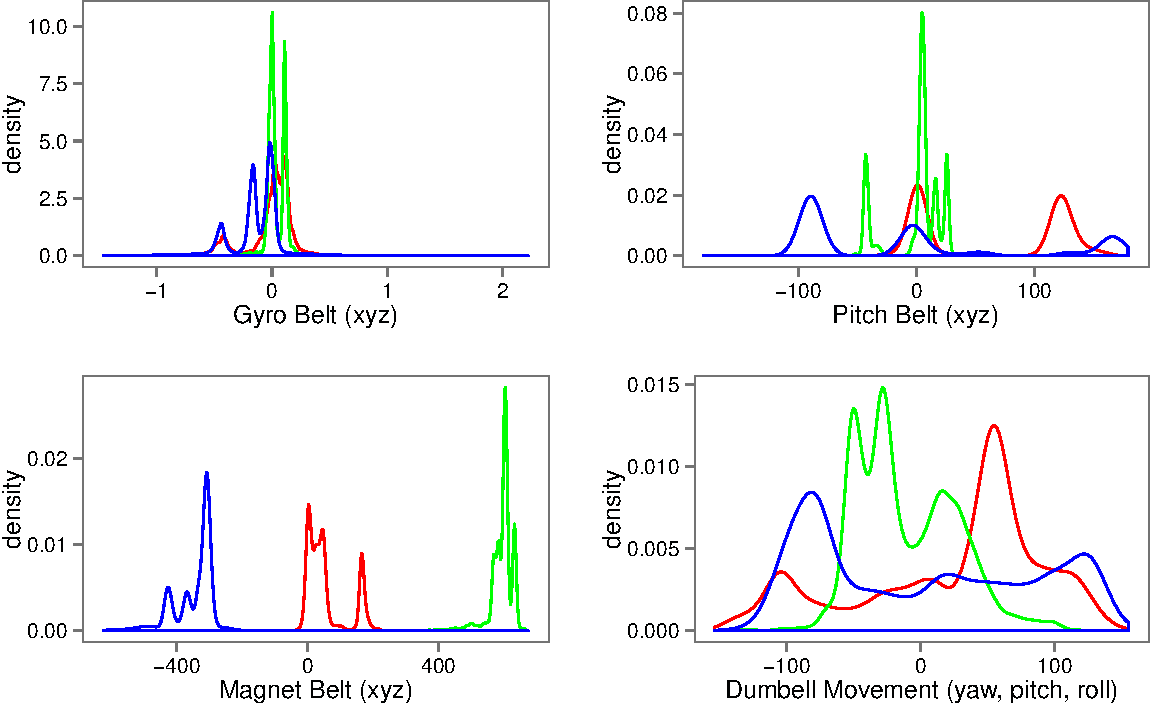
\includegraphics{MLproject_files/figure-latex/unnamed-chunk-2-1} \end{center}

\textbf{Partitioning the Data}

The dataset was partitioned into training and testing datasets, with
60\% of the original data going to the training set and 40\% to the
testing set. The model was built with the training dataset, then tested
on the testing dataset. The following code performs this procedure:

\begin{Shaded}
\begin{Highlighting}[]
\CommentTok{# partition training dataset into 60/40 train/test}
\NormalTok{train_part =}\StringTok{ }\KeywordTok{createDataPartition}\NormalTok{(train_used$classe, }\DataTypeTok{p =} \FloatTok{0.6}\NormalTok{, }\DataTypeTok{list =} \OtherTok{FALSE}\NormalTok{)}
\NormalTok{training =}\StringTok{ }\NormalTok{train_used[train_part, ]}
\NormalTok{testing =}\StringTok{ }\NormalTok{train_used[-train_part, ]}
\NormalTok{##}
\end{Highlighting}
\end{Shaded}

\textbf{The Model}

Many methods of classification were attempted, including niave Bayes,
multinomial logistic regression, and Support Vector Machines. It was
determined that the Random Forest method produced the best results. In
addition, pre-processing using principal component analysis was
attempted however this greatly reduced the prediction accuracy.

Cross validation was not used, as, according to the creators of the
Random Forest algorithm Leo Breiman and Adele Cutler, there is no need
for cross-validation. See
\url{http://www.stat.berkeley.edu/~breiman/RandomForests/cc_home.htm\#ooberr}
for more information.

The R code is shown below, as is the confusion matrix. The out of the
bag error rate in the training and the confusion matrix is shown below.
For informational purposes a plot of the error rate versus number of
trees is also shown.

\begin{Shaded}
\begin{Highlighting}[]
\KeywordTok{set.seed}\NormalTok{(}\DecValTok{1777}\NormalTok{)}
\NormalTok{random_forest=}\KeywordTok{randomForest}\NormalTok{(classe~.,}\DataTypeTok{data=}\NormalTok{training,}\DataTypeTok{ntree=}\DecValTok{500}\NormalTok{,}\DataTypeTok{importance=}\OtherTok{TRUE}\NormalTok{)}
\NormalTok{random_forest}
\end{Highlighting}
\end{Shaded}

\begin{verbatim}
## 
## Call:
##  randomForest(formula = classe ~ ., data = training, ntree = 500,      importance = TRUE) 
##                Type of random forest: classification
##                      Number of trees: 500
## No. of variables tried at each split: 7
## 
##         OOB estimate of  error rate: 0.72%
## Confusion matrix:
##      A    B    C    D    E  class.error
## A 3346    1    0    1    0 0.0005973716
## B   12 2258    9    0    0 0.0092145678
## C    0   23 2028    3    0 0.0126582278
## D    0    0   25 1903    2 0.0139896373
## E    0    0    3    6 2156 0.0041570439
\end{verbatim}

\begin{Shaded}
\begin{Highlighting}[]
\KeywordTok{plot}\NormalTok{(random_forest,}\DataTypeTok{main=}\StringTok{"Random Forest: Error Rate vs Number of Trees"}\NormalTok{)}
\end{Highlighting}
\end{Shaded}

\begin{center}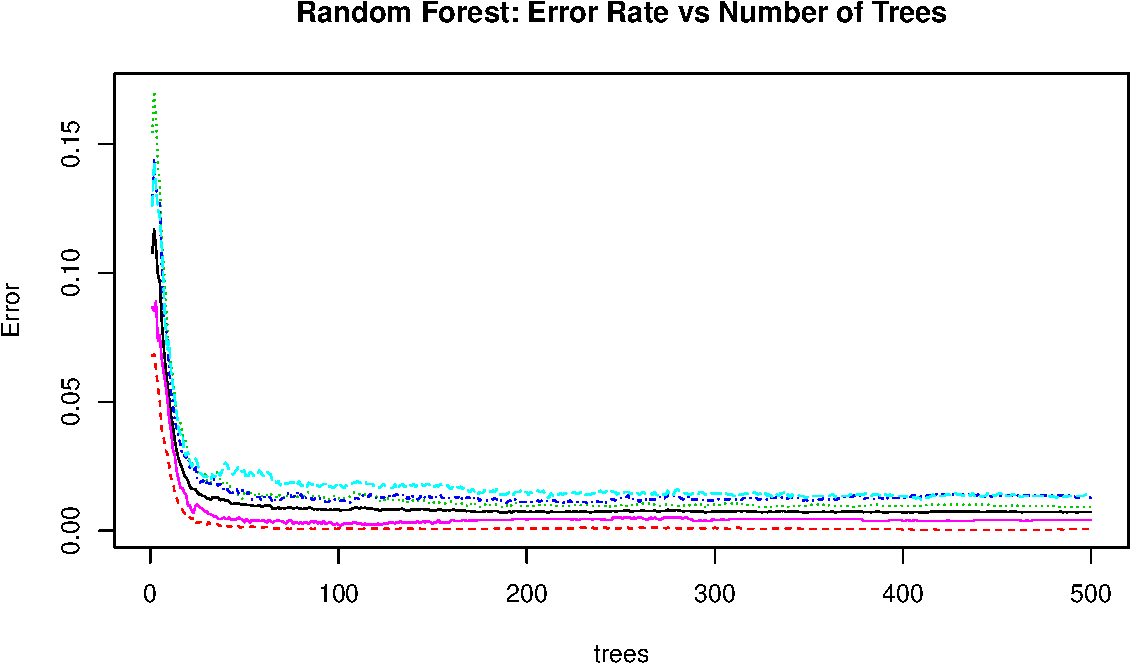
\includegraphics{MLproject_files/figure-latex/unnamed-chunk-4-1} \end{center}

\textbf{Variable Importance}

It may be of interest to know which variables were most `important' in
the building of the model. This can be seen by plotting the mean
decrease in accuracy and the mean decrease in the Gini coefficient per
variable. In short, the more the accuracy of the random forest decreases
due to the exclusion (or permutation) of a single variable, the more
important that variable is deemed to be. The mean decrease in the Gini
coefficient is a measure of how each variable contributes to the
homogeneity of the nodes and leaves in the resulting random forest.
(from
\url{https://dinsdalelab.sdsu.edu/metag.stats/code/randomforest.html})

\begin{Shaded}
\begin{Highlighting}[]
\NormalTok{imp=}\KeywordTok{importance}\NormalTok{(random_forest)}
\NormalTok{impL=imp[,}\KeywordTok{c}\NormalTok{(}\DecValTok{6}\NormalTok{,}\DecValTok{7}\NormalTok{)]}
\NormalTok{imp.ma=}\KeywordTok{as.matrix}\NormalTok{(impL)}
\NormalTok{imp.df=}\KeywordTok{data.frame}\NormalTok{(imp.ma)}

\KeywordTok{write.csv}\NormalTok{(imp.df, }\StringTok{"imp.df.csv"}\NormalTok{, }\DataTypeTok{row.names=}\OtherTok{TRUE}\NormalTok{)}
\NormalTok{imp.df.csv=}\KeywordTok{read.csv}\NormalTok{(}\StringTok{"imp.df.csv"}\NormalTok{,}\DataTypeTok{header=}\OtherTok{TRUE}\NormalTok{)}

\KeywordTok{colnames}\NormalTok{(imp.df.csv)=}\KeywordTok{c}\NormalTok{(}\StringTok{"Variable"}\NormalTok{,}\StringTok{"MeanDecreaseAccuracy"}\NormalTok{,}\StringTok{"MeanDecreaseGini"}\NormalTok{)}
\NormalTok{imp.sort =}\StringTok{  }\NormalTok{imp.df.csv[}\KeywordTok{order}\NormalTok{(-imp.df.csv$MeanDecreaseAccuracy),] }

\NormalTok{imp.sort =}\StringTok{ }\KeywordTok{transform}\NormalTok{(imp.df.csv, }
  \DataTypeTok{Variable =} \KeywordTok{reorder}\NormalTok{(Variable, MeanDecreaseAccuracy))}

\NormalTok{VIP=}\KeywordTok{ggplot}\NormalTok{(}\DataTypeTok{data=}\NormalTok{imp.sort, }\KeywordTok{aes}\NormalTok{(}\DataTypeTok{x=}\NormalTok{Variable, }\DataTypeTok{y=}\NormalTok{MeanDecreaseAccuracy)) +}\StringTok{ }
\StringTok{  }\KeywordTok{ylab}\NormalTok{(}\StringTok{"Mean Decrease Accuracy"}\NormalTok{)+}\KeywordTok{xlab}\NormalTok{(}\StringTok{""}\NormalTok{)+}
\StringTok{    }\KeywordTok{geom_bar}\NormalTok{(}\DataTypeTok{stat=}\StringTok{"identity"}\NormalTok{,}\DataTypeTok{fill=}\StringTok{"skyblue"}\NormalTok{,}\DataTypeTok{alpha=}\NormalTok{.}\DecValTok{8}\NormalTok{,}\DataTypeTok{width=}\NormalTok{.}\DecValTok{75}\NormalTok{)+}\StringTok{ }
\StringTok{    }\KeywordTok{coord_flip}\NormalTok{()+}\KeywordTok{theme_few}\NormalTok{() }

\NormalTok{imp.sort.Gini <-}\StringTok{ }\KeywordTok{transform}\NormalTok{(imp.df.csv, }
                      \DataTypeTok{Variable =} \KeywordTok{reorder}\NormalTok{(Variable, MeanDecreaseGini))}

\NormalTok{VIP.Gini=}\KeywordTok{ggplot}\NormalTok{(}\DataTypeTok{data=}\NormalTok{imp.sort.Gini, }\KeywordTok{aes}\NormalTok{(}\DataTypeTok{x=}\NormalTok{Variable, }\DataTypeTok{y=}\NormalTok{MeanDecreaseGini)) +}\StringTok{ }
\StringTok{  }\KeywordTok{ylab}\NormalTok{(}\StringTok{"Mean Decrease Gini"}\NormalTok{)+}\KeywordTok{xlab}\NormalTok{(}\StringTok{""}\NormalTok{)+}
\StringTok{  }\KeywordTok{geom_bar}\NormalTok{(}\DataTypeTok{stat=}\StringTok{"identity"}\NormalTok{,}\DataTypeTok{fill=}\StringTok{"skyblue"}\NormalTok{,}\DataTypeTok{alpha=}\NormalTok{.}\DecValTok{8}\NormalTok{,}\DataTypeTok{width=}\NormalTok{.}\DecValTok{75}\NormalTok{)+}\StringTok{ }
\StringTok{  }\KeywordTok{coord_flip}\NormalTok{()+}\KeywordTok{theme_few}\NormalTok{() }

\NormalTok{VarImpPlot=}\KeywordTok{arrangeGrob}\NormalTok{(VIP, VIP.Gini,}\DataTypeTok{ncol=}\DecValTok{2}\NormalTok{)}
\KeywordTok{grid.draw}\NormalTok{(VarImpPlot)}
\end{Highlighting}
\end{Shaded}

\begin{center}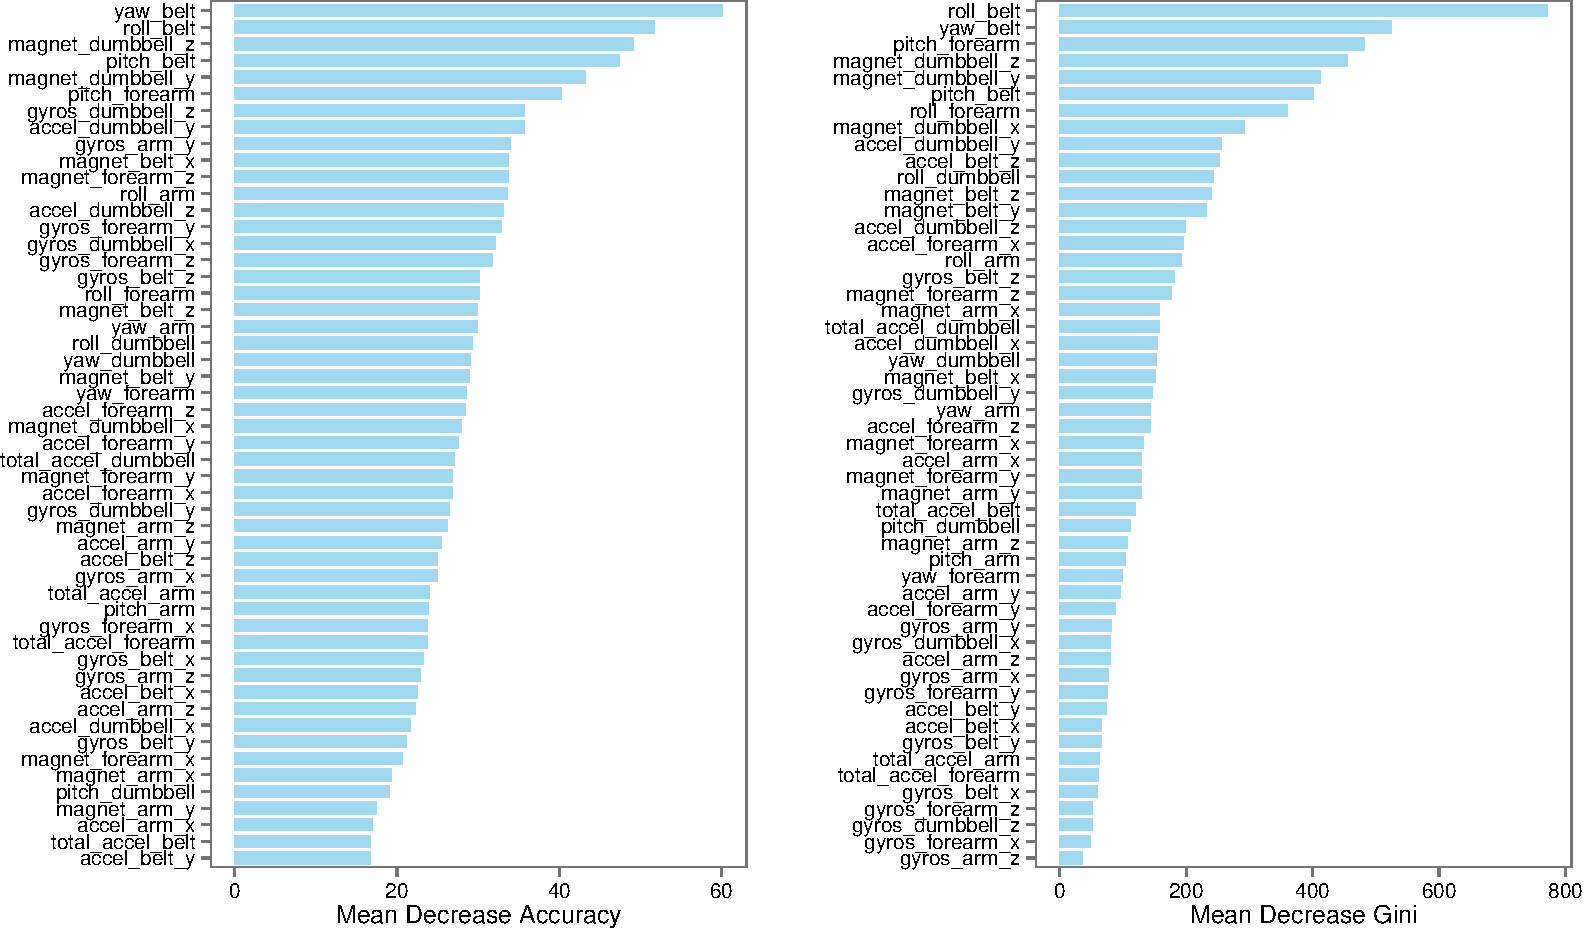
\includegraphics{MLproject_files/figure-latex/unnamed-chunk-5-1} \end{center}

\textbf{Model Applied to Testing Dataset}

\begin{Shaded}
\begin{Highlighting}[]
\NormalTok{test_predictions =}\StringTok{ }\KeywordTok{predict}\NormalTok{(random_forest, }\DataTypeTok{newdata=}\NormalTok{testing)}
\NormalTok{CM =}\StringTok{ }\KeywordTok{confusionMatrix}\NormalTok{(test_predictions,testing$classe)}
\NormalTok{CM}
\end{Highlighting}
\end{Shaded}

\begin{verbatim}
## Confusion Matrix and Statistics
## 
##           Reference
## Prediction    A    B    C    D    E
##          A 2231   15    0    0    0
##          B    1 1495   16    0    0
##          C    0    8 1352   16    0
##          D    0    0    0 1270    4
##          E    0    0    0    0 1438
## 
## Overall Statistics
##                                           
##                Accuracy : 0.9924          
##                  95% CI : (0.9902, 0.9942)
##     No Information Rate : 0.2845          
##     P-Value [Acc > NIR] : < 2.2e-16       
##                                           
##                   Kappa : 0.9903          
##  Mcnemar's Test P-Value : NA              
## 
## Statistics by Class:
## 
##                      Class: A Class: B Class: C Class: D Class: E
## Sensitivity            0.9996   0.9848   0.9883   0.9876   0.9972
## Specificity            0.9973   0.9973   0.9963   0.9994   1.0000
## Pos Pred Value         0.9933   0.9888   0.9826   0.9969   1.0000
## Neg Pred Value         0.9998   0.9964   0.9975   0.9976   0.9994
## Prevalence             0.2845   0.1935   0.1744   0.1639   0.1838
## Detection Rate         0.2843   0.1905   0.1723   0.1619   0.1833
## Detection Prevalence   0.2863   0.1927   0.1754   0.1624   0.1833
## Balanced Accuracy      0.9984   0.9911   0.9923   0.9935   0.9986
\end{verbatim}

The model was applied to the testing dataset and generated predictions
for the class of weightlifting type. Above is the code that was used and
the confusion matrix for the testing dataset. The accuracy is very high,
\(0.9924\). The model accurately predicted all of the 20 test subjects.

\textbf{Cross Validation}

Just in case the grader feels it is necessary to do cross validation, I
have added the code and error rates from the CV from the caret package.
The cross-validation error is shown below. The model with CV leads to
slightly poorer performance than the previous one.

\begin{Shaded}
\begin{Highlighting}[]
\NormalTok{CV =}\StringTok{ }\KeywordTok{trainControl}\NormalTok{(}\DataTypeTok{method =} \StringTok{"cv"}\NormalTok{, }\DataTypeTok{number =} \DecValTok{5}\NormalTok{, }\DataTypeTok{allowParallel =} \NormalTok{T, }\DataTypeTok{verboseIter =} \NormalTok{F)}
\NormalTok{CVmodel =}\StringTok{ }\KeywordTok{train}\NormalTok{(classe ~}\StringTok{ }\NormalTok{., }\DataTypeTok{data =} \NormalTok{training, }\DataTypeTok{method =} \StringTok{"rf"}\NormalTok{, }\DataTypeTok{prox =} \NormalTok{F, }\DataTypeTok{trControl =} \NormalTok{CV)}
\NormalTok{CVmodel}
\end{Highlighting}
\end{Shaded}

\begin{verbatim}
## Random Forest 
## 
## 11776 samples
##    52 predictor
##     5 classes: 'A', 'B', 'C', 'D', 'E' 
## 
## No pre-processing
## Resampling: Cross-Validated (5 fold) 
## Summary of sample sizes: 9421, 9421, 9421, 9420, 9421 
## Resampling results across tuning parameters:
## 
##   mtry  Accuracy   Kappa      Accuracy SD  Kappa SD   
##    2    0.9875171  0.9842075  0.002374385  0.003003771
##   27    0.9877720  0.9845300  0.002499365  0.003162878
##   52    0.9800448  0.9747543  0.005153059  0.006523229
## 
## Accuracy was used to select the optimal model using  the largest value.
## The final value used for the model was mtry = 27.
\end{verbatim}

\begin{Shaded}
\begin{Highlighting}[]
\NormalTok{predsCVmodel =}\StringTok{ }\KeywordTok{predict}\NormalTok{(CVmodel, }\DataTypeTok{newdata =} \NormalTok{testing)}

\NormalTok{confMatrix =}\StringTok{ }\KeywordTok{confusionMatrix}\NormalTok{(predsCVmodel,testing$classe)}
\NormalTok{confMatrix}
\end{Highlighting}
\end{Shaded}

\begin{verbatim}
## Confusion Matrix and Statistics
## 
##           Reference
## Prediction    A    B    C    D    E
##          A 2227   17    0    0    0
##          B    3 1484   22    1    0
##          C    1   16 1337   20    2
##          D    0    1    9 1265    7
##          E    1    0    0    0 1433
## 
## Overall Statistics
##                                           
##                Accuracy : 0.9873          
##                  95% CI : (0.9845, 0.9896)
##     No Information Rate : 0.2845          
##     P-Value [Acc > NIR] : < 2.2e-16       
##                                           
##                   Kappa : 0.9839          
##  Mcnemar's Test P-Value : NA              
## 
## Statistics by Class:
## 
##                      Class: A Class: B Class: C Class: D Class: E
## Sensitivity            0.9978   0.9776   0.9773   0.9837   0.9938
## Specificity            0.9970   0.9959   0.9940   0.9974   0.9998
## Pos Pred Value         0.9924   0.9828   0.9717   0.9867   0.9993
## Neg Pred Value         0.9991   0.9946   0.9952   0.9968   0.9986
## Prevalence             0.2845   0.1935   0.1744   0.1639   0.1838
## Detection Rate         0.2838   0.1891   0.1704   0.1612   0.1826
## Detection Prevalence   0.2860   0.1925   0.1754   0.1634   0.1828
## Balanced Accuracy      0.9974   0.9867   0.9857   0.9905   0.9968
\end{verbatim}

\end{document}
